
%% bare_conf.tex
%% V1.3
%% 2007/01/11
%% by Michael Shell
%% See:
%% http://www.michaelshell.org/
%% for current contact information.
%%
%% This is a skeleton file demonstrating the use of IEEEtran.cls
%% (requires IEEEtran.cls version 1.7 or later) with an IEEE conference paper.
%%
%% Support sites:
%% http://www.michaelshell.org/tex/ieeetran/
%% http://www.ctan.org/tex-archive/macros/latex/contrib/IEEEtran/
%% and
%% http://www.ieee.org/

%%*************************************************************************
%% Legal Notice:
%% This code is offered as-is without any warranty either expressed or
%% implied; without even the implied warranty of MERCHANTABILITY or
%% FITNESS FOR A PARTICULAR PURPOSE!
%% User assumes all risk.
%% In no event shall IEEE or any contributor to this code be liable for
%% any damages or losses, including, but not limited to, incidental,
%% consequential, or any other damages, resulting from the use or misuse
%% of any information contained here.
%%
%% All comments are the opinions of their respective authors and are not
%% necessarily endorsed by the IEEE.
%%
%% This work is distributed under the LaTeX Project Public License (LPPL)
%% ( http://www.latex-project.org/ ) version 1.3, and may be freely used,
%% distributed and modified. A copy of the LPPL, version 1.3, is included
%% in the base LaTeX documentation of all distributions of LaTeX released
%% 2003/12/01 or later.
%% Retain all contribution notices and credits.
%% ** Modified files should be clearly indicated as such, including  **
%% ** renaming them and changing author support contact information. **
%%
%% File list of work: IEEEtran.cls, IEEEtran_HOWTO.pdf, bare_adv.tex,
%%                    bare_conf.tex, bare_jrnl.tex, bare_jrnl_compsoc.tex
%%*************************************************************************

% *** Authors should verify (and, if needed, correct) their LaTeX system  ***
% *** with the testflow diagnostic prior to trusting their LaTeX platform ***
% *** with production work. IEEE's font choices can trigger bugs that do  ***
% *** not appear when using other class files.                            ***
% The testflow support page is at:
% http://www.michaelshell.org/tex/testflow/



% Note that the a4paper option is mainly intended so that authors in
% countries using A4 can easily print to A4 and see how their papers will
% look in print - the typesetting of the document will not typically be
% affected with changes in paper size (but the bottom and side margins will).
% Use the testflow package mentioned above to verify correct handling of
% both paper sizes by the user's LaTeX system.
%
% Also note that the "draftcls" or "draftclsnofoot", not "draft", option
% should be used if it is desired that the figures are to be displayed in
% draft mode.
%
\documentclass[10pt, conference, compsocconf]{IEEEtran}
% Add the compsocconf option for Computer Society conferences.
%
% If IEEEtran.cls has not been installed into the LaTeX system files,
% manually specify the path to it like:
% \documentclass[conference]{../sty/IEEEtran}





% Some very useful LaTeX packages include:
% (uncomment the ones you want to load)
\usepackage{color}
\usepackage{colortbl}

\definecolor{lightgray}{gray}{.95}
\definecolor{darkgray}{gray}{.80}

\usepackage{epsfig}
\usepackage{listings}

\usepackage{array}
\usepackage{longtable}
\usepackage{hhline}
\usepackage{listings}
%\usepackage{tabular}

\lstset{ %
lineskip=0.5pt,
basicstyle=\scriptsize,       % the size of the fonts that are used for the code
%numbers=left,                   % where to put the line-numbers
numberstyle=\scriptsize,      % the size of the fonts that are used for the line-numbers
stepnumber=1,                   % the step between two line-numbers. If it is 1 each line will be numbered
numbersep=3pt,                  % how far the line-numbers are from the code
backgroundcolor=\color{lightgray},  % choose the background color. You must add \usepackage{color}
showspaces=false,               % show spaces adding particular underscores
showstringspaces=false,         % underline spaces within strings
showtabs=false,                 % show tabs within strings adding particular underscores
frame=none,                   % adds a frame around the code
tabsize=2,              % sets default tabsize to 2 spaces
captionpos=b,                   % sets the caption-position to bottom
breaklines=true,        % sets automatic line breaking
breakatwhitespace=false,    % sets if automatic breaks should only happen at whitespace
escapeinside={\%}{)}          % if you want to add a comment within your code
}


% *** MISC UTILITY PACKAGES ***
%
%\usepackage{ifpdf}
% Heiko Oberdiek's ifpdf.sty is very useful if you need conditional
% compilation based on whether the output is pdf or dvi.
% usage:
% \ifpdf
%   % pdf code
% \else
%   % dvi code
% \fi
% The latest version of ifpdf.sty can be obtained from:
% http://www.ctan.org/tex-archive/macros/latex/contrib/oberdiek/
% Also, note that IEEEtran.cls V1.7 and later provides a builtin
% \ifCLASSINFOpdf conditional that works the same way.
% When switching from latex to pdflatex and vice-versa, the compiler may
% have to be run twice to clear warning/error messages.






% *** CITATION PACKAGES ***
%
\usepackage{cite}
% cite.sty was written by Donald Arseneau
% V1.6 and later of IEEEtran pre-defines the format of the cite.sty package
% \cite{} output to follow that of IEEE. Loading the cite package will
% result in citation numbers being automatically sorted and properly
% "compressed/ranged". e.g., [1], [9], [2], [7], [5], [6] without using
% cite.sty will become [1], [2], [5]--[7], [9] using cite.sty. cite.sty's
% \cite will automatically add leading space, if needed. Use cite.sty's
% noadjust option (cite.sty V3.8 and later) if you want to turn this off.
% cite.sty is already installed on most LaTeX systems. Be sure and use
% version 4.0 (2003-05-27) and later if using hyperref.sty. cite.sty does
% not currently provide for hyperlinked citations.
% The latest version can be obtained at:
% http://www.ctan.org/tex-archive/macros/latex/contrib/cite/
% The documentation is contained in the cite.sty file itself.






% *** GRAPHICS RELATED PACKAGES ***
%
\ifCLASSINFOpdf
  % \usepackage[pdftex]{graphicx}
  % declare the path(s) where your graphic files are
  % \graphicspath{{../pdf/}{../jpeg/}}
  % and their extensions so you won't have to specify these with
  % every instance of \includegraphics
  % \DeclareGraphicsExtensions{.pdf,.jpeg,.png}
\else
  % or other class option (dvipsone, dvipdf, if not using dvips). graphicx
  % will default to the driver specified in the system graphics.cfg if no
  % driver is specified.
  % \usepackage[dvips]{graphicx}
  % declare the path(s) where your graphic files are
  % \graphicspath{{../eps/}}
  % and their extensions so you won't have to specify these with
  % every instance of \includegraphics
  % \DeclareGraphicsExtensions{.eps}
\fi
% graphicx was written by David Carlisle and Sebastian Rahtz. It is
% required if you want graphics, photos, etc. graphicx.sty is already
% installed on most LaTeX systems. The latest version and documentation can
% be obtained at:
% http://www.ctan.org/tex-archive/macros/latex/required/graphics/
% Another good source of documentation is "Using Imported Graphics in
% LaTeX2e" by Keith Reckdahl which can be found as epslatex.ps or
% epslatex.pdf at: http://www.ctan.org/tex-archive/info/
%
% latex, and pdflatex in dvi mode, support graphics in encapsulated
% postscript (.eps) format. pdflatex in pdf mode supports graphics
% in .pdf, .jpeg, .png and .mps (metapost) formats. Users should ensure
% that all non-photo figures use a vector format (.eps, .pdf, .mps) and
% not a bitmapped formats (.jpeg, .png). IEEE frowns on bitmapped formats
% which can result in "jaggedy"/blurry rendering of lines and letters as
% well as large increases in file sizes.
%
% You can find documentation about the pdfTeX application at:
% http://www.tug.org/applications/pdftex





% *** MATH PACKAGES ***
%
%\usepackage[cmex10]{amsmath}
% A popular package from the American Mathematical Society that provides
% many useful and powerful commands for dealing with mathematics. If using
% it, be sure to load this package with the cmex10 option to ensure that
% only type 1 fonts will utilized at all point sizes. Without this option,
% it is possible that some math symbols, particularly those within
% footnotes, will be rendered in bitmap form which will result in a
% document that can not be IEEE Xplore compliant!
%
% Also, note that the amsmath package sets \interdisplaylinepenalty to 10000
% thus preventing page breaks from occurring within multiline equations. Use:
%\interdisplaylinepenalty=2500
% after loading amsmath to restore such page breaks as IEEEtran.cls normally
% does. amsmath.sty is already installed on most LaTeX systems. The latest
% version and documentation can be obtained at:
% http://www.ctan.org/tex-archive/macros/latex/required/amslatex/math/





% *** SPECIALIZED LIST PACKAGES ***
%
%\usepackage{algorithmic}
% algorithmic.sty was written by Peter Williams and Rogerio Brito.
% This package provides an algorithmic environment fo describing algorithms.
% You can use the algorithmic environment in-text or within a figure
% environment to provide for a floating algorithm. Do NOT use the algorithm
% floating environment provided by algorithm.sty (by the same authors) or
% algorithm2e.sty (by Christophe Fiorio) as IEEE does not use dedicated
% algorithm float types and packages that provide these will not provide
% correct IEEE style captions. The latest version and documentation of
% algorithmic.sty can be obtained at:
% http://www.ctan.org/tex-archive/macros/latex/contrib/algorithms/
% There is also a support site at:
% http://algorithms.berlios.de/index.html
% Also of interest may be the (relatively newer and more customizable)
% algorithmicx.sty package by Szasz Janos:
% http://www.ctan.org/tex-archive/macros/latex/contrib/algorithmicx/




% *** ALIGNMENT PACKAGES ***
%
%\usepackage{array}
% Frank Mittelbach's and David Carlisle's array.sty patches and improves
% the standard LaTeX2e array and tabular environments to provide better
% appearance and additional user controls. As the default LaTeX2e table
% generation code is lacking to the point of almost being broken with
% respect to the quality of the end results, all users are strongly
% advised to use an enhanced (at the very least that provided by array.sty)
% set of table tools. array.sty is already installed on most systems. The
% latest version and documentation can be obtained at:
% http://www.ctan.org/tex-archive/macros/latex/required/tools/


%\usepackage{mdwmath}
%\usepackage{mdwtab}
% Also highly recommended is Mark Wooding's extremely powerful MDW tools,
% especially mdwmath.sty and mdwtab.sty which are used to format equations
% and tables, respectively. The MDWtools set is already installed on most
% LaTeX systems. The lastest version and documentation is available at:
% http://www.ctan.org/tex-archive/macros/latex/contrib/mdwtools/


% IEEEtran contains the IEEEeqnarray family of commands that can be used to
% generate multiline equations as well as matrices, tables, etc., of high
% quality.


%\usepackage{eqparbox}
% Also of notable interest is Scott Pakin's eqparbox package for creating
% (automatically sized) equal width boxes - aka "natural width parboxes".
% Available at:
% http://www.ctan.org/tex-archive/macros/latex/contrib/eqparbox/





% *** SUBFIGURE PACKAGES ***
%\usepackage[tight,footnotesize]{subfigure}
% subfigure.sty was written by Steven Douglas Cochran. This package makes it
% easy to put subfigures in your figures. e.g., "Figure 1a and 1b". For IEEE
% work, it is a good idea to load it with the tight package option to reduce
% the amount of white space around the subfigures. subfigure.sty is already
% installed on most LaTeX systems. The latest version and documentation can
% be obtained at:
% http://www.ctan.org/tex-archive/obsolete/macros/latex/contrib/subfigure/
% subfigure.sty has been superceeded by subfig.sty.



%\usepackage[caption=false]{caption}
%\usepackage[font=footnotesize]{subfig}
% subfig.sty, also written by Steven Douglas Cochran, is the modern
% replacement for subfigure.sty. However, subfig.sty requires and
% automatically loads Axel Sommerfeldt's caption.sty which will override
% IEEEtran.cls handling of captions and this will result in nonIEEE style
% figure/table captions. To prevent this problem, be sure and preload
% caption.sty with its "caption=false" package option. This is will preserve
% IEEEtran.cls handing of captions. Version 1.3 (2005/06/28) and later
% (recommended due to many improvements over 1.2) of subfig.sty supports
% the caption=false option directly:
%\usepackage[caption=false,font=footnotesize]{subfig}
%
% The latest version and documentation can be obtained at:
% http://www.ctan.org/tex-archive/macros/latex/contrib/subfig/
% The latest version and documentation of caption.sty can be obtained at:
% http://www.ctan.org/tex-archive/macros/latex/contrib/caption/




% *** FLOAT PACKAGES ***
%
%\usepackage{fixltx2e}
% fixltx2e, the successor to the earlier fix2col.sty, was written by
% Frank Mittelbach and David Carlisle. This package corrects a few problems
% in the LaTeX2e kernel, the most notable of which is that in current
% LaTeX2e releases, the ordering of single and double column floats is not
% guaranteed to be preserved. Thus, an unpatched LaTeX2e can allow a
% single column figure to be placed prior to an earlier double column
% figure. The latest version and documentation can be found at:
% http://www.ctan.org/tex-archive/macros/latex/base/



%\usepackage{stfloats}
% stfloats.sty was written by Sigitas Tolusis. This package gives LaTeX2e
% the ability to do double column floats at the bottom of the page as well
% as the top. (e.g., "\begin{figure*}[!b]" is not normally possible in
% LaTeX2e). It also provides a command:
%\fnbelowfloat
% to enable the placement of footnotes below bottom floats (the standard
% LaTeX2e kernel puts them above bottom floats). This is an invasive package
% which rewrites many portions of the LaTeX2e float routines. It may not work
% with other packages that modify the LaTeX2e float routines. The latest
% version and documentation can be obtained at:
% http://www.ctan.org/tex-archive/macros/latex/contrib/sttools/
% Documentation is contained in the stfloats.sty comments as well as in the
% presfull.pdf file. Do not use the stfloats baselinefloat ability as IEEE
% does not allow \baselineskip to stretch. Authors submitting work to the
% IEEE should note that IEEE rarely uses double column equations and
% that authors should try to avoid such use. Do not be tempted to use the
% cuted.sty or midfloat.sty packages (also by Sigitas Tolusis) as IEEE does
% not format its papers in such ways.



\usepackage{boxedminipage}
\usepackage{graphicx}

\newcommand{\notesbox}[1]{
%     \ \\
      \noindent\begin{center}\begin{boxedminipage}[h]{0.4\textwidth}{#1}\end{boxedminipage}\end{center}
}

% *** PDF, URL AND HYPERLINK PACKAGES ***
%
%\usepackage{url}
% url.sty was written by Donald Arseneau. It provides better support for
% handling and breaking URLs. url.sty is already installed on most LaTeX
% systems. The latest version can be obtained at:
% http://www.ctan.org/tex-archive/macros/latex/contrib/misc/
% Read the url.sty source comments for usage information. Basically,
% \url{my_url_here}.

% *** Do not adjust lengths that control margins, column widths, etc. ***
% *** Do not use packages that alter fonts (such as pslatex).         ***
% There should be no need to do such things with IEEEtran.cls V1.6 and later.
% (Unless specifically asked to do so by the journal or conference you plan
% to submit to, of course. )


% correct bad hyphenation here
\hyphenation{op-tical net-works semi-conduc-tor}


\begin{document}
%
% paper title
% can use linebreaks \\ within to get better formatting as desired
\title{ARC - Automatic Repair of Concurrency Bugs}


% author names and affiliations
% use a multiple column layout for up to two different
% affiliations

\author{\IEEEauthorblockN{Kevin Jalbert, David Kelk, Jeremy S. Bradbury}
\IEEEauthorblockA{Software Quality Research Group\\
Faculty of Science (Computer Science)\\
University of Ontario Institute of Technology\\
Oshawa, Ontario, Canada\\
\{kevin.jalbert, david.kelk, jeremy.bradbury\}@uoit.ca}
}

% conference papers do not typically use \thanks and this command
% is locked out in conference mode. If really needed, such as for
% the acknowledgment of grants, issue a \IEEEoverridecommandlockouts
% after \documentclass

% for over three affiliations, or if they all won't fit within the width
% of the page, use this alternative format:
%
%\author{\IEEEauthorblockN{Michael Shell\IEEEauthorrefmark{1},
%Homer Simpson\IEEEauthorrefmark{2},
%James Kirk\IEEEauthorrefmark{3},
%Montgomery Scott\IEEEauthorrefmark{3} and
%Eldon Tyrell\IEEEauthorrefmark{4}}
%\IEEEauthorblockA{\IEEEauthorrefmark{1}School of Electrical and Computer Engineering\\
%Georgia Institute of Technology,
%Atlanta, Georgia 30332--0250\\ Email: see http://www.michaelshell.org/contact.html}
%\IEEEauthorblockA{\IEEEauthorrefmark{2}Twentieth Century Fox, Springfield, USA\\
%Email: homer@thesimpsons.com}
%\IEEEauthorblockA{\IEEEauthorrefmark{3}Starfleet Academy, San Francisco, California 96678-2391\\
%Telephone: (800) 555--1212, Fax: (888) 555--1212}
%\IEEEauthorblockA{\IEEEauthorrefmark{4}Tyrell Inc., 123 Replicant Street, Los Angeles, California 90210--4321}}




% use for special paper notices
%\IEEEspecialpapernotice{(Invited Paper)}




% make the title area
\maketitle


\begin{abstract}

Automatic repair of single-threaded programs is being realised in practice.
Similar progress has not been made on the automatic repair of parallel
programs.  We introduce a fully automated two-phase system for repairing
deadlocks and data races in parallel Java programs. The approach works on any
Java source code and requires only rudimentary test cases. Annotations, formal
specifications or other notations are not required. As only the concurrency
mechanisms are targeted the semantic meaning of the program is not changed. In
the first phase an evolutionary strategy is used to mutate the existing program
until a variant is found that fixes the deadlocks and data races. As the first
phase may introduce unneeded synchronization, a second phase attempts to
optimize performance by removing the excess synchronization without sacraficing
program correctness. We describe the approach and report on early results.

\end{abstract}

\begin{IEEEkeywords}
concurrency; genetic programming; mutation.

\end{IEEEkeywords}


% For peer review papers, you can put extra information on the cover
% page as needed:
% \ifCLASSOPTIONpeerreview
% \begin{center} \bfseries EDICS Category: 3-BBND \end{center}
% \fi
%
% For peerreview papers, this IEEEtran command inserts a page break and
% creates the second title. It will be ignored for other modes.
\IEEEpeerreviewmaketitle



\section{Introduction}
\label{sec:introduction}

As desktop computers now ship with more than one processor, programs must
parallelize to continue to benefit from Moore's Law. Inevitibly these programs
contain bugs. If fixing bugs in single-threaded programs is a difficult
and resource intensive task,  it is doubly so in multi-threaded programs.
Parallelism~\cite{SL05} introduces new classes of bugs and makes them harder to
find by having them only occur in rare execution interleavings~\cite{MQB07}.
Data-races cause variables to take on unpredictable values as different threads
race to write to them while deadlocks bring part or all of a running program to
a halt.

We propose ARC (Automatic Repair of Concurrency bugs): An automatic technique
to repair deadlocks and data races in parallel Java programs. Formal
specifications, annotations and elaborate test suites are not required. Only
the Java source code and test(s) demonstrating the deadlocks and data races are
necessary. Evolutionary strategies are used to evolve variants until one is
found that fixes the bugs in question.

There has been a great deal of research in the area of search-based software
engineering~\cite{Har+10}. Furthermore, the use of heuristic search to identify
a solution fixing a bug is not a novel idea~\cite{FNWG09, AY08, Arc08, WT10,
WNLF09, WFGN10}. Our proposed approach adapts the original idea of
automatically fixing sequential programs to specifically target concurrent
software.

Evolutionary strategies (ES) is part of the family of heuristic search
algorithms. They are population-based technique driven by mutation. Crossover
and replacement are not used.  All members of the population exist throughout
an invocation of the search. A fitness function is used to evaluate each
member's proposed fix. Bugs in a concurrent program are fixed by iteratively
mutating the program and evaluating each mutation by executing the program many
times. IBM's ConTest~\cite{EFN+02} is used to explore different interleavings
of the program under test to increase our confidence bugs are not slipping by.
Fitness improves with the number of correct executions.

Large search spaces are a problem faced by all bug fixing techniques.
Parallelism introduces thread interleavings on top of this. A number of steps
are taken to address this issue.  First, we limit the algorithm to only fixing
deadlocks and data races. Second, only the concurrency mechanisms are targeted.
Specifically, \textit{synchronize} statements are added, removed, swapped,
grown and shrunk. No other statements are affected. Third, we use a specific
set of eleven TXL~\cite{CHP91} operators based on the ConMan
operators~\cite{BCD06} to mutate the code.

ARC operates in two phases. In the first, synchronized blocks are added,
expanded and swapped to attempt to fix the bugs. This may add unnecessary
synchronization. If a correct program is found in phase one, a second phase  is
run where synchronization blocks are shrunk or removed in an attempt to
increase efficiency. As this can introduce data races or deadlocks, any mutant
decreasing correctness is rejected.

To the best of our knowledge there has been no previous work using evolutionary
strategies to fix bugs in concurrent software.  There has been work involving
the correction of concurrency bugs using self-healing~\cite{LVK08}. From the
paper, \textit{The healing techniques based on influencing the scheduling do
not guarantee that a detected problem will really be completely removed, but
they can decrease the probability of its manifestation.} In contrast ARC is an
off-line technique that fixes the bug by modifying the source code.

The main contributions of this paper are:

\begin{itemize}

\item An algorithm to create minimal fixes for deadlocks and data races in Java
programs. Only the source code and tests demonstrating the bugs are necessary.
To the best of our knowledge this is the first approach to fix both kinds of
bugs in Java programs.

\item Methods to constrain the search space: Specific targeting of
synchronization mechanisms and the TXL operators implementing this.

\end{itemize}


\subsection{Motivation using quote from GenProg paper}
\begin{quote}\textit{Some properties are difficult or impossible to encode
using test cases, such as nondeterministic properties; GenProg cannot
currently repair race conditions, for example.}~\cite{GNFW11}
\end{quote}

\section{Background}
\label{sec:background}

All of the material discussed here revolves around the topics of concurrency,
model checking, heuristic search and state-space exploration. A firm
understanding of these topics is required for various parts of the paper.

\subsection{Concurrency}
\label{sec:concurrency}

Concurrency is the act of having multiple threads executing in parallel.
Threads in programs are objects which execute statements. Concurrent programs 
are able to exploit multi-core systems as threads can be distributed across
each of the CPUs to increase performance. Concurrency introduces a new class
class of bugs, the \textit{heisenbugs}.  Due to concurrent access to shared 
memory, threads are able to cause \textit{dataraces} and \textit{deadlocks}.

A \textbf{data race} has been defined as: \textit{``\ldots two or more
concurrent threads access a shared variable and when at least one access is a
write, and the threads use no explicit mechanism to prevent the access from
being simultaneous.''}~\cite{LSW07}

A \textbf{deadlock} as: \textit{``\ldots a situation where two or more
processes are unable to proceed because each is waiting for one of the others
to do something in a deadlock cycle \ldots} For example, this occurs when a
thread holds a lock that another thread desires and vice-versa''~\cite{LSW07}

These bugs are extremely difficult to detect due to the non-deterministic
nature of how threads are interleaved (the way the system schedules them). In
one execution a concurrency bug might occur, then a second, third and forth it
does not. Various techniques are available to try and detect concurrency bugs
such as static analysis~\cite{NA07,NPSG09,HP04}, stress testing~\cite{HSU03},
dynamic analysis~\cite{JNPS09,EFN+02}, and model
checking~\cite{BHPV00,RDH03,OM03,MQB07,Holz97,JM04,HP00}.

\subsection{Evolutionary Programming}
\label{sec:evolutionary_programming}

Evolutionary programming (EP) is part of the family of heuristic search
algorithms. The most commonly referenced heuristic search technique is the
genetic algorithm~\cite{GA92}. For space reasons only the briefest outline of
EP and it's place in the heuristic search family is given.

A standard genetic algorithm is population based, uses mutation, crossover
and a fitness function to evolve solutions to problems. A proposed solution to
the problem is encoded as a member of the population. Each is evaluated by a
fitness function.   The more fit a member solution is, the greater the chance
it will pass it's genetic material (solution) on to the next generation.
\textit{Selection pressure prefentially selects better solutions.} Crossover
mixes these solutions to produce new solutions while mutation injects fresh
information in to the population so it doesn't become stagnant.

EP is a simpler form of search than a genetic algorithm. A population of
proposed solutions is generated and mutated each generation.  Crossover and
selection aren't used, so the same population exists throughout the evolution.
Every members fitness is evaluated every generation. It ends when a
predetermined fitness is reached or after a set number of generations have
passed.

Why use mutation only?  Sometimes it is unclear how to use crossover.  For
example, if the member solutions are Java programs, how does one ensure that
when putting two halves of different programs together the resulting program is
correct, makes sense or even compiles?

\section{Related Works}
\label{sec:related_works}

There are a number of approaches to automatically hide or fix bugs in programs.
Attempts to fix single-threaded and multi-threaded software are looked at
in turn.

Co-evolutionary competition between programs with bugs and test cases is used
in~\cite{AY08, Arc08, WT10}. Both approaches use genetic programming to evolve
fixes. Co-evolution is used to cause competition between the evolving fixes and
test cases. In both cases the resulting framework is tested only againt a toy
sorting algorithm with mixed success. The untargeted nature of the fixing
process is the largest limitation. No effort is made to constrain the large
search space of the problem.

Significant improvements on the previous approach are made in~\cite{FNWG09,
WNLF09, NWLF09, WFGN10, GNFW11}. Formal specifications are no longer required.
Instead, test cases are used to demonstrate the bug and describe the desired
functionality that must be preserved. To address the limitations of the
previous approach they introduce two innovations: First, they assume the bug is
written correctly in  another part of the program. Second, they determine the
error path on which the bug occurs and target those statements specifically for
repair.  Together these additions constrain the state space enough that the
framework can fix real bugs in real programs.

Similar to the work done here,~\cite{KLT+07, LVK08} uses ConTest to heal data
races. From their paper, \textit{``Healing concurrency problems is about
limiting or changing the probability of interleaving, such that bugs will be
seen less.''} In contrast, our approach uses ConTest to fix both data races and
deadlocks.

A framework is created in~\cite{CB05} to ``repair'' buffer overflow attacks.
When one is identified, the program state is reset to what it was before the
attack. The attack packet is disgarded then the program continues running. As
in the previous approach the goal is to hide the problem, not fix it.

SAT solving is used in~\cite{AY07}  to repair shared memory concurrent programs
``w.r.t. CTL specifications'' where processes atomically read, write one shared
variable at a time. All that is required is the concurrent program and a
specification in modal or temporal logic. It is unclear if the fix is applied
to the program or the specification of the program.

\section{Motivating Problem}
\label{sec:motivation}

As described above, concurrency bugs are difficult to detect and fix. Many
tools exist that identify concurrent bugs. The identification of a problem is
often not enough as multiple code fragments are involved, possibly in different
units with differently named variables. In this ambiguous scenario the 
appropriate fix is not always clear. There has been work in concurrency 
anti-patterns that provide a definition, problem, context and solution for 
concurrency bugs~\cite{BJ09}.

For example, we have a \texttt{write} and \texttt{read} method accessing a
shared variable. A very simple data race bug exists because there is no atomic
access to the \texttt{data} variable during the reading or writing. Both
methods are involved in the data race, and it is because of the interactions 
between these methods that a data race is possible. The solution involves 
synchronizing both accesses (as shown in Figure~\ref{fig:fixed_sample_datarace}). 
Synchronizing one method does not fix the bug.

This solution, is far from ideal as it forces other threads to wait while the
write method works on the loop and database sections. An optimization is to
shrink the critical region (the synchronized statements) to only guard access
to the shared variable (as shown in
Figure~\ref{fig:optimized_sample_datarace}).

\begin{figure}[!h]
\vspace{2mm}
\begin{minipage}{3.70cm}
\footnotesize{\textbf{Buggy Program:}}
\begin{lstlisting}[language=Java]
write(int var1){
  ... // Expensive loop
  data = var1;
  ... // Database query
}

int public read(){
  return data;
}
\end{lstlisting}
\end{minipage}\hfill
\begin{minipage}{3.70cm}
\footnotesize{\textbf{Fixed Program:}}
\begin{lstlisting}[language=Java]
synchronize write(int var1){
  ... // Expensive loop
  data = var1;
  ... // Database query
}

int synchronize read(){
  return data;
}
\end{lstlisting}
\end{minipage}
\caption{A developer first synchronizes the \texttt{read} function, yet the bug
still presents itself. Synchronizing the \texttt{write} method as well fixes
the bug.}
\label{fig:fixed_sample_datarace}
\end{figure}

\begin{figure}[!h]
\vspace{2mm}
\begin{minipage}{3.70cm}
\footnotesize{\textbf{$1^{st}$ Optimization on Fix:}}
\begin{lstlisting}[language=Java]
public write(int var1){
  ... // Expensive loop
  synchronized(this){
    data = var1;
    ... // Database query
  }
}

int synchronize read(){
  return data;
}
\end{lstlisting}
\end{minipage}\hfill
\begin{minipage}{3.70cm}
\footnotesize{\textbf{$2^{nd}$ Optimization on Fix:}}
\begin{lstlisting}[language=Java]
public write(int var1){
  ... // Expensive loop
  synchronized(this){
    data = var1;
  }
  ... // Database query
}

int synchronize read(){
  return data;
}
\end{lstlisting}
\end{minipage}
\caption{A developer first shrinks the critical region to exclude the expensive
loop. They shrink the critical region again to exclude the database query as a
further optimization.}
\label{fig:optimized_sample_datarace}
\end{figure}

From a developer's standpoint there is a lot of work involved in creating a fix
for parallel bugs as multiple changes are not uncommon. As the example
illustrated, two changes were required to functionally fix the program. Two
additional changes were required to improve the non-functional performance.

Automated tools in software testing and debugging are needed as they have the
potential to reduce the vast amount of resources spent on software testing
(upwards to \$59.5 billion)~\cite{RTI02}. ARC provides an automated approach to
first fixing the \textit{functionality}, and then optimizing the \textit{non-
functional} performance of programs with concurrency bugs.

\section{ARC's Approach}
\label{sec:approach}

Essentially ARC aims to automatically repair concurrency bugs like the one
presented in Section~\ref{sec:motivation}. A high-level overview of ARC's
approach is presented in Figure~\ref{fig:process}. There are two inputs to ARC,
firstly the buggy program and secondly a comprehensive JUnit testsuite. This
testsuite is necessary as it acts like an oracle in determining if the bug
still exists in the program. One limitation of ARC is that it can only fix bugs
that can be detected by the testsuite, thus a comprehensive testsuite is
required.

\begin{figure}[!h]
  \centering
  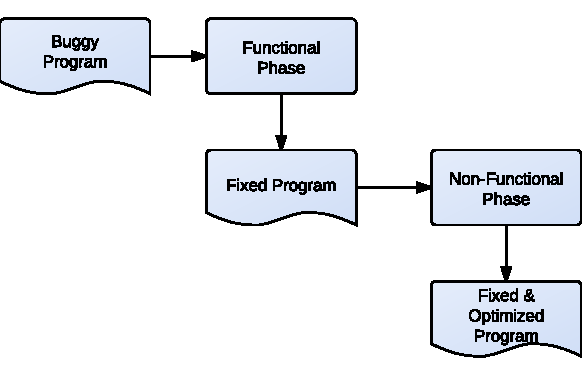
\includegraphics[width=7.0cm]{figures/process.pdf}
  \caption{High Level Overview of ARC's Repair and Optimization Process}
  \label{fig:process}
\end{figure}

ARC is composed of two major phases, the \textit{Functional Phase} and the
\textit{Non-Functional Phase}. Both phases are similar in terms of the steps
they follow, though there are slight variations to accomplish different goals.
As ARC is using an evolutionary algorithm, the first phase attempts to fix the
buggy program while the second phase attempts to optimize the fixed program
produced from the previous phase. The result of the last phase is a fixed
program that is functionally fixed and that the non-functional performance is
optimized. The next set of sections will detail each step of the phases (as
shown in Figure~\ref{fig:phases_internals}) all while indicating the
differences in each phase.

As ARC uses an evolutionary algorithm to evolve solutions from the buggy
program, the key aspects of the approach is the mutation and evaluation steps.

\begin{figure}[!h]
  \centering
  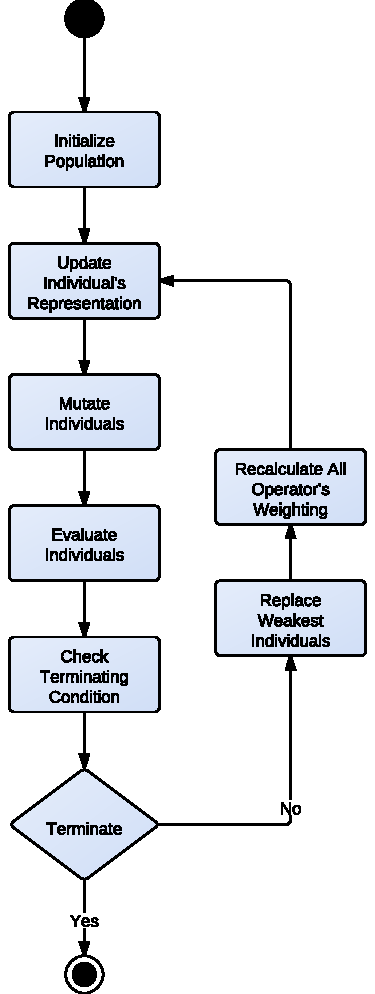
\includegraphics[width=4.50cm]{figures/phases.pdf}
  \caption{Internal View of ARC's Phases}
  \label{fig:phases_internals}
\end{figure}

\subsection{Initialize Population}
\label{sec:initialize_population}

Before ARC can start with either phase it must initialize the population of
individuals. The initialization of individuals involves creating a copy of the
program so that the rest of the phase can mutate these copies. In the
functional phase the original buggy program is copied into each individual. For
the non-functional phase ARC would have already produced the fixed program as a
result of the functional phase, thus each individual receives a copy of the
fixed program.

\subsection{Update Individual's Representation}
\label{sec:update_individual_representation}

An individual will be mutated from generation-to-generation based off of its
current representation. Therefore this step will update the represent based on
the individual's state of the program. The individual's representation consists
of an array each with a set of variable elements, with each array representing
a particular mutation operator and each element representing an instance found
in the program. Table~\ref{tbl:individual_representation} illustrates the
program representation. Further details of selecting and applying mutation are
covered in the next section.

As ARC is mutating the concurrency aspects of this program the program changes
in concurrency structure through mutation. Essentially the search space of
possible mutations is changing every generation. This is why the representation
must be updated to account for this.

Based on the individual's current version of the program that is being evolved,
there exists a set of possible mutations that can occur. Each mutation will
result in new possible locations that can be mutated, thus we need to update
the individual's representation to account for the changing set of mutation
operators.

\begin{table}[!h]
\begin{center}
\begin{tabular}{|l|l|}
\hline
\textbf{Operator} &
\textbf{Instances}
\\\hline
Mutation 1 & 0
\\\hline
Mutation 2 & 0 0 0
\\\hline
Mutation 3 & --
\\\hline
\ldots & \ldots
\\\hline
Mutation $n$ & 0 0
\\\hline
\end{tabular}
\caption{Example representation of an individual, each 0 represents an instance
of where the operator can be applied. There can be up to $n$ mutation operators
with no-limit to the number of instances per operator.}
\label{tbl:individual_representation}
\end{center}
\end{table}

\subsection{Mutate Individuals}
\label{sec:mutate_individuals}

As suggested at in the previous section, the mutation step will attempt to
mutate each individual's current program state. The mutation step begins with
selecting a mutation operator, then by selecting an instance using the
individual's representation. When these two options are selected then the
mutation is applied and the program's state has changed.

The set of mutation operators are listed in Table~\ref{tbl:operators}. These
mutation operators are TXL operators, specifically they are derived from the
ConMAn operators~\cite{BCD06}. TXL operators work by looking for a pattern and then
transforming it according to a set of rules, and example of one of our
operators is shown in Figure~\ref{fig:EXSB_example}.

\begin{table*}
\begin{center}
\begin{tabular}{|l|l|c|c|}
\hline
\textbf{Operator} &
\textbf{Acronym} &
\textbf{Functional} &
\textbf{Non-Functional}
\\\hline
Add synch. around synch. & ASAS & $\surd$ &
\\\hline
Add synch. around variable & ASAV & $\surd$ &
\\\hline
Add synch. around method & ASM & $\surd$ &
\\\hline
Change synch. order & CSO & $\surd$ &
\\\hline
Expand synch. before & EXSB & $\surd$ &
\\\hline
Expand synch. after & EXSA & $\surd$ &
\\\hline
Remove synch. around synch. & RSAS & $\surd$ & $\surd$
\\\hline
Remove synch. around variable & RSAV & $\surd$ & $\surd$
\\\hline
Remove synch. around method & RSM & $\surd$ & $\surd$
\\\hline
Remove synch. around block & RSB & $\surd$ & $\surd$
\\\hline
Shrink synch. before & SHSB & & $\surd$
\\\hline
Shrink synch. after & SHSA & & $\surd$
\\\hline
\end{tabular}
\caption{Set of mutation operators used by ARC, indicating which phases they
are considered in for possible mutations.}
\label{tbl:operators}
\end{center}
\end{table*}

\begin{figure}[h!]
\vspace{2mm}
\begin{minipage}{3.70cm}

\footnotesize{\textbf{ Program $P$:}}
\begin{lstlisting}[language=Java]
  ...
  obj.write(var1);
  synchronized(lock){
    myHash.remove(var1);
  }
\end{lstlisting}
\end{minipage}\hfill
\begin{minipage}{3.70cm}
\footnotesize{\textbf{ Program $P'$:}}
\begin{lstlisting}[language=Java]
  ...
  synchronized(lock){
    obj.write(var1);
    myHash.remove(var1);
  }
\end{lstlisting}
\end{minipage}

\caption{Example of EXSB, the expand synchronization before operator.}
\label{fig:EXSB_example}
\end{figure}

Evolutionary strategies (ES) are solely mutation driven. During the fixing
phase ARC adds, expands and alters synchronization blocks in an attept to fix
deadlocks and data races. During the second phase ARC attempts to shrink and
remove synchronization to improve performance. Table~\ref{tbl:operators} lists
the operators used in ARC by phase.

Mutation is a multi-step process. Each member of the ES population contains
it's own copy of the Java project to be fixed.  During the mutation phase each
TXL operator operates against each source code unit to create all mutants of
it's type. For example, the expand synchronization before (EXSB,
Table~\ref{fig:EXSB_example}) operator is applied to every existing concurrency
block in every Java file. All mutants - where each concurrency block is
expanded at the front by one statement - are exaustively written to separate
files. This is repeated for every Java file in the project and each elidgeable
mutant available in the phase.

With all mutants written to files, an operator is randomly selected to become
the actual mutation operator for that member project for that generation.  One
of it's mutations is randomly selected and applied to the project as the actual
mutation.

Note that each member project must have it's mutants tracked separately as the
application of mutations causes the points where future mutation occur to
diverge.  (If a synchronization block is added to the first project, EXSB,
EXSA, SHSB and SHSA can operate on it in future generations. The second project
may expand an existing synchronization and so-on.)

Statistics are gathered on the performance of each operator.  After a
defineable number of generations a weighting scheme is applied:  Mutation
operators that were more successful in the past are given higher weights so
they are more likely to be selected in the current generation.  Weightings are
designed to insure the chance of selection is always greater than zero
regardless of performance.  A sliding window is used to dynamically update the
weights as the evolution progresses.

(This goes somewhere else?) As ARC only adds, removes and changes
synchronization blocks, the meaning of a program shouldn't change.

\subsection{Evaluate Individuals}
\label{sec:evalute_individuals}
Each individual is now at a new program state, thus they are evaluated to
determine whether they are in a better state or not.  In the functional phase
the evaluation criteria is based on the success of test cases. In the
non-functional phase the evaluation criteria is based on the performance of the
program, with the condition that it continues to perform the same according the
functional phase's evaluation criteria.

\subsection{Check Terminating Condition}
\label{sec:check_terminating_condition}

Each phase will continue to evolve and evaluate individuals until some
terminating condition is met. After the evaluation of each individual the
terminating conditions are checked, the following conditions are for the
functional phase:

\begin{enumerate}
  \item A solution is found (100\% successful executions)
  \item No solution is found within the generational limit
  \item The population has converged (no improvement has been seen in $x$ generations)
\end{enumerate}

For the non-functional phase the terminating conditions are the same as the
functional phase except for the first one. This condition is dropped because
there is no actual best known solution for optimal performance unlike a fixes
program in the functional phase.

In the situation where no terminating condition is met then the process will
contiue to operating in that phase. If condition is met then the best found
individual represents the output of the phase.

\subsection{Replace Weakest Individuals}
\label{sec:replace_weakest_individuals}
With any evolutionary algorithm it is entirely possible for an individual to
stray down a path that leads to little or no improvement. To encourage
individuals to explore more of the potential states we employ a replacement
strategy that replaces the lower $x$ percentage of individuals with a random
individual that resides in the upper $x$ percent.  These replacements only
occur after an individual has seen at least $y$ new changes. In addition, we
feel that the original state of the bug is not too far from the solution. To
prevent individuals from straying to far from the original state an individual
is reseted to the original state if the individual has not seen any improvement
in $z$ generations.
% TODO Double check that ARC actually does it like this

\subsection{Recalculate All Operator's Weighting}
\label{sec:recalculate_operator_weighting}
ARC utilizes a heuristic approach for selecting the mutation operator in the
mutation step. A sliding window of $n$ generations is used while figuring out
the success of previously used mutation operators. If certain mutation
operators tend to improve individuals fitness score, then we want to utilize
these mutation operators more then ones that have not seen such success. The
sliding window is used to prevent domination of the weighting. To ensure that
this approach is up to date the current weighting for each operator is
recalculated based on the new feedback received from the population.

\subsection{Fitness Functions}
\label{sec:fitness_functions}

A key problem in parallel programming is the unpredictability of thread
interleavings.  If a parallel bug appears only rarely, how can we gain
confidence that a proposed fix actually works?  IBM's ConTest
Tool~\cite{EFN+02} is used to instrument the project and inject noise into it's
scheduled interleavings. ConTest is then invoked by ARC many times to test each
member program in turn. By running ConTest multiple times we gain confidence
enough interleavings are explored to find bugs. Note that running ConTest many
times for each member of the population at each generation is time intensive.

In the first phase fitness is determined by the number of successfull ConTest
runs. In the first phase fitness is determined by the number of successful
ConTest runs. We consider timeouts as they could either result in a deadlock or
a successful execution given more time.

\begin{figure}
\begin{footnotesize}
\begin{center}
$functional\ fitness(P) = (s \times sw) + (t \times tw)$
\end{center}
\end{footnotesize}
\begin{tiny}
\begin{center}
$s = \#\ of\ successful\ executions$ \\
$sw = success\ weighting$ \\
$t = \#\ of\ timeout\ executions$ \\
$tw = timeout\ weighting$
\end{center}
\end{tiny}
\caption{Fitness Function for Functional Phase}
\label{fig:functional_fitness}
\end{figure}

Phase one ends when a ES member is found that passes all ConTest runs. There is
a possibility that the bug isn't truly fixed in the proposed solution.  (By
chance the proper interleavings were not explored.)  ARC has an additional
safeguard for this:  Every proposed fix is run a large number of times in
ConTest. (The default is 10x more runs than a ES member experiences in any
generation.) If any test fails the solution is rejected and the evolutionary
process continues.

Once a fix is found the second phase begins.  Here the fitness function is
concerned with optimizing performance.  Fitness is now determined by the wall
time required for an execution and the number of voluntary context switches
made.  Durning the initialization of phase 2 the proposed fix is run a large
number of times to determine baseline averages for these two values.

\begin{figure}
\begin{footnotesize}
\begin{center}
$non-functional\ fitness(P) = \frac{worst\ score}{[sig_t \times unc(t)] + [sig_c \times unc(c)]}$
\end{center}
\vspace{0.1cm} \textit{Where:} \vspace{0.1cm}
\end{footnotesize}
\begin{tiny}
\begin{center}
$unc(x) = \frac{(x_{max} - x_{min})}{x_{avg}}$ \\ \vspace{0.2cm}
$
  sig_t = \left\{
  \begin{array}{l l}
    t/c & \quad if\ t\ > c \\
    c/t & \quad if\ c\ > t \\
  \end{array} \right.
$ \\ \vspace{0.2cm}
$
  sig_s = \left\{
  \begin{array}{l l}
    c/t & \quad if\ t\ > c \\
    t/c & \quad if\ c\ > t \\
  \end{array} \right.
$ \\
\end{center}
\end{tiny}
\caption{Fitness Function for Non-Functional Phase}
\label{fig:nonfunctional_fitness}
\end{figure}

We reason these two metrics are important as excessive synchronization causes
contention within a program. Contention causes it to take longer. Contention
will also increase the amount of yielding/context switches in a program. Phase
two attempts to reduce contention by removing and reducing synchronization.

Removing and reducing synchronization runs the risk of introducing new bugs in
to the program. Before every phase 2 fitness evaluation is performed, a phase 1
fitness evaluation is performed again.  If any deadlock or data race is
encountered the proposed fix is rejected.  That member has it's project reset
to it's state in the previous generation.

Assuming correctness hasn't suffered the member program is run again a number
of times in ConTest.  Average wall time and voluntary context switches are
computed and compared to the baseline values.  Improvements are rewarded with
higher fitness.

As it isn't clear when a member program is as optimized as it could be - and
there is no a-priori way to know this, the second phase runs for it's full
allotment of generations.  At the end it outputs the member program with the
highest non-functional fitness (from any generation) as the final optimized
fix.

\section{Experiments}
\label{sec:experiments}

ARC is designed to automatically repair concurrency bugs. A proper
evaluation must measure ARC's ability to do so. We are also interesting in how
efficient ARC is at finding these solutions.

Due to the repairing and optimization nature of ARC it is entirely possible for
a program to perform better or worst then it originally performed. We are
also interested in the effect of performance of the solution produced by ARC.

\subsection{Experimental Setup}
\label{sec:experimental_setup}

Programs were are going to evaluate ARC on come from the IBM
Concurrency Benchmark~\cite{EHSU06}. This set of programs are rather small yet
demonstrate a variety of concurrency bug types. None of them contain the required
test suite.  They were manually created without altering the programs and their
bugs. Details on the programs are presented in Table~\ref{tbl:used_programs}.

\begin{table}[!h]
\begin{center}
\begin{tabular}{|l|r|r|l|}
\hline
\textbf{Program} &
\textbf{SLOC} &
\textbf{Classes} &
\textbf{Bug Type}
\\\hline
Deadlock2 & 38 & 1 & Deadlock
\\\hline
Account & 164 & 3 & Data race
\\\hline
AirlineBug & 89 & 1 & Data race
\\\hline
AllocationVector & 161 & 3 & Data race
\\\hline
Buffer & 324 & 5 & ?
\\\hline
BubbleSort & 237 & 4 & ?
\\\hline
Deadlock & 107 & 2 & Deadlock
\\\hline
BufWriter& 168 & 5 & ?
\\\hline
BankAccounts & 75 & 2 & ?
\\\hline
Pingpong & 142 & 4 & ?
\\\hline
\end{tabular}
\caption{The set of used programs to evaluate ARC. The testsuite for each
program is excluded from these values.}
\label{tbl:used_programs}
\end{center}
\end{table}

ARC was designed to be flexible in terms of the parameters that can be
configured. Table~\ref{tbl:used_parameters} lists and describes each parameter,
including the values selected for evaluation. Values were selected based on
our experience with ARC.

\begin{table*}[!t]
\begin{center}
\begin{tabular}{|p{3cm}|p{10cm}|r|}
\hline
\textbf{Parameter} &
\textbf{Description} &
\textbf{Value}
\\\hline
Project Test Mb & The amount of memory allocated for the testing & 2048
\\\hline
ConTest Runs & The number of testsuite executions performed in the evaluation phase & 50
\\\hline
ConTest Timeout Seconds & The amount of time in seconds that a testsuite execution will last before a timeout occurs & 20
\\\hline
Evolution Generations & The maximum number of generations that can occur within each phase  & 100
\\\hline
Evolution Population & The size of the population for the evolutionary algorithms, a collection of individuals& 80
\\\hline
Evolution Replace Lowest Percent & The scoring individuals that reside below the given percent of the population will be replaced/restarted & 10
\\\hline
Evolution Replace With Best Percent & The replaced individuals will be replaced with the best individual of the population with the given percent, otherwise it is restarted & 60
\\\hline
Evolution Replace Interval & The replacement of lowest individuals only occurs on the specified generational intervals & 10
\\\hline
Dynamic Ranking Window & The number of generations that are considered (in a sliding window fashion) when re-evaluating the weighting of mutation operators in terms of their successes & 10
\\\hline
Success Weight & The weighting applied for successful executions during the functional phase's evaluation & 100
\\\hline
Timeout Weight & The weighting applied for timeout executions during the functional phase's evaluation & 10
\\\hline
Generational Improvement Window & This specifies the size of the sliding window that check for convergence of the population & 10
\\\hline
Average Fitness Min Delta & When checking for convergence this represents the minimum acceptable delta for the average fitness of the population & 5
\\\hline
Best Fitness Min Delta & When checking for convergence this represents the minimum acceptable delta for the best fitness of the population & 5 % TODO Does this actually look in the specific generation or over all generations? 
\\\hline
\end{tabular}
\caption{The set of parameters that ARC uses along with their descriptions and
used values for the experimentations.}
\label{tbl:used_parameters}
\end{center}
\end{table*}

\subsection{Experimental Results}
\label{sec:experimental_results}

Each program was run through ARC a total of 10 times using the parameters 
described in Table~\ref{tbl:used_parameters}. The results of each
program is summarized in Table~\ref{tbl:summary_results}.

\begin{table*}[!t]
\begin{center}
\begin{tabular}{|p{2cm}|p{0.6cm}|p{1.75cm}|p{2cm}|p{2cm}|p{2cm}|p{2cm}|}
\hline
\textbf{Program} &
\textbf{\% of Fixes} &
\textbf{Range of Fix Containing Generation} &
\textbf{Range of Original's Execution Time (s)} &
\textbf{Range of Solution's Execution Time (s)} &
\textbf{Range of Original's \# of Context Switches} &
\textbf{Range of Solution's \# of Context Switches}
\\\hline
Deadlock2 & 0.6 & [3--17] & [0.10--0.14] & [0.9--0.12] & [73--97] & [60--81]
\\\hline
Account & 0.6 & [3--17] & [0.10--0.14] & [0.9--0.12] & [73--97] & [60--81]
\\\hline
AirlineBug & 0.6 & [3--17] & [0.10--0.14] & [0.9--0.12] & [73--97] & [60--81]
\\\hline
AllocationVector & 0.6 & [3--17] & [0.10--0.14] & [0.9--0.12] & [73--97] & [60--81]
\\\hline
Buffer & 0.6 & [3--17] & [0.10--0.14] & [0.9--0.12] & [73--97] & [60--81]
\\\hline
BubbleSort & 0.6 & [3--17] & [0.10--0.14] & [0.9--0.12] & [73--97] & [60--81]
\\\hline
Deadlock & 0.6 & [3--17] & [0.10--0.14] & [0.9--0.12] & [73--97] & [60--81]
\\\hline
BufWriter & 0.6 & [3--17] & [0.10--0.14] & [0.9--0.12] & [73--97] & [60--81]
\\\hline
BankAccounts & 0.6 & [3--17] & [0.10--0.14] & [0.9--0.12] & [73--97] & [60--81]
\\\hline
Pingpong & 0.6 & [3--17] & [0.10--0.14] & [0.9--0.12] & [73--97] & [60--81]
\\\hline
\end{tabular}
\caption{Summary of the results of running the programs (Table~\ref{tbl:used_programs}) through ARC 10 times.}
\label{tbl:summary_results}
\end{center}
\end{table*}




\section{Threats to Validity}




\section{Future Work}
\label{sec:future_work}

Currently ARC mutates all variables of the program under test. Ideally it
should target only those involved in concurrency. We believe there are off-the-
shelf solutions integrateable into ARC to give it this capability, similar
to~\cite{CM08, HP00}.

Targeting the variables, functions and classes on the error path is another
feature we would like to add.  It has shown great success in helping to isolate
and automatically fix bugs in single-threaded programs~\cite{FNWG09, NWLF09,
WFGN10, GNFW11}. We believe it will do the same for multithreaded programs.

Generalizing the TXL operators is also important. Currently the add
synchronization around synchronization operator (ASAS) for example, only adds
\texttt{synchronize(this) \{...\}} to the Java source.  When the analysis of
the previous two paragraphs are implemented the operators need to be updated to
work with them.

We also plan to experiment with new operators.  Potential additions include
splitting or merging synchronization blocks and changing the argument in the
synchronize call.

Many new concurrency structures were introduced in Java 5. Expanding ARC's
operators to deal with new anti-patterns~\cite{BJ09, BCD06} gives ARC the 
ability to fix additional types of bugs.

\section{Conclusion}
\label{sec:conclusion}

We identified a lack of automated repair techniques in the literature.
Concurrency bugs were identified as a difficult bug to automatically repair
using exists techniques. We developed an approach that uses an evolutionary
algorithm to evolve a buggy program into one that fixes the bug identified
through a testsuite. Our technique operators in two phases, the first being to
fix the program while the second is to optimize the performance.

An experiment was conducted to evaluate ARC using a set of 10 programs found in
a concurrency benchmark. The results indicate that ARC is \ldots % TODO

% use section* for acknowledgement
%\section*{Acknowledgment}
%The authors would like to thank the Natural Sciences and Engineering Research Council of Canada (NSERC) for funding this research.


% trigger a \newpage just before the given reference
% number - used to balance the columns on the last page
% adjust value as needed - may need to be readjusted if
% the document is modified later
%\IEEEtriggeratref{8}
% The "triggered" command can be changed if desired:
%\IEEEtriggercmd{\enlargethispage{-5in}}

% references section

% can use a bibliography generated by BibTeX as a .bbl file
% BibTeX documentation can be easily obtained at:
% http://www.ctan.org/tex-archive/biblio/bibtex/contrib/doc/
% The IEEEtran BibTeX style support page is at:
% http://www.michaelshell.org/tex/ieeetran/bibtex/
\bibliographystyle{IEEEtran}
% argument is your BibTeX string definitions and bibliography database(s)
\bibliography{x2012}
%
% <OR> manually copy in the resultant .bbl file
% set second argument of \begin to the number of references
% (used to reserve space for the reference number labels box)

% that's all folks
\end{document}
